\documentclass[11pt]{article}
\usepackage{tocloft}
\usepackage{graphicx}
\usepackage{calc}
\usepackage{amssymb}
\usepackage{color}
\usepackage{array}
\usepackage[sc]{mathpazo}
\usepackage{url}
\usepackage[final]{pdfpages}
\usepackage{amsmath}

%\linespread{1.05}
\oddsidemargin=0pt
\evensidemargin=0pt
\textwidth=6.5in
\topmargin=0pt
\headheight=0pt
\headsep=0pt
\textheight=9in
% EXPERIMENTAL
%\parindent=0pt
%\parskip=3pt
\setlength{\parindent}{0cm}
\newcommand\secfont{\fontfamily{cmss}\selectfont}%\textwidth 5.5truein
\newcommand\pifheading[1]{{\secfont\textbf{#1}:}}
%\oddsidemargin -0.40truein
%\textheight 8.0truein
%\topmargin -0.25truein
\def\lo{
\mathrel{\raise.3ex\hbox{$<$}\mkern-14mu\lower0.6ex\hbox{$\sim$}}
}
\def\hi{
\mathrel{\raise.3ex\hbox{$>$}\mkern-14mu\lower0.6ex\hbox{$\sim$}}
}

\textwidth = 6.6 in
\textheight = 9.1 in
\oddsidemargin = -0.05 in
\evensidemargin = +0.05 in
\topmargin = -.1 in
\headheight = 0.0 in
\headsep = 0.0 in
\parskip = 0.06in
\newcommand\registered{{\ooalign{\hfil\raise .00ex\hbox{\scriptsize R}\hfil\crcr\mathhexbox20D}}}

%% Define a new 'leo' style for the package that will use a smaller font.
\makeatletter
\def\url@leostyle{%
  \@ifundefined{selectfont}{\def\UrlFont{\sf}}{\def\UrlFont{\small\ttfamily}}}
\makeatother
%% Now actually use the newly defined style.
\urlstyle{leostyle}

%\pagestyle{empty}
%\includeonly{previous,proposal_references}
%\includeonly{proposal_references}
%\includeonly{previous}

% TOC

\begin{document}
\pagenumbering{gobble}
%%%%%%%%%%%%%%%%%%%%%%%%%%%%%%%%%%%%%%%%%%%%%%%%%%%%%%%%%%%%%%%%%%%%%
\begin{center}
\textbf{\Large
AST101: Our Place in the Universe \\
\vspace*{0.1cm}
Lab 11: Radioactive Decay with Dice 
}
\end{center}

\vspace*{0.5cm}

{\Large Name:}\vspace*{0.5cm}\\\hrule
{\Large Partners:}\vspace*{0.5cm}\\\hrule
{\Large Lab section:}\vspace*{0.5cm}\\\hrule
\vspace*{0.5cm}

%%%%%%%%%%%%%%%%%%%%%%%%%%%%%%%%%%%%%%%%%%%%%%%%%%%%%%%%%%%%%%%%%%%%%
\section{Introduction}

Many kinds of nuclei are {\it radioactive}: randomly, over time, they change into other kinds, spitting out high-energy nuclear radiation as they do so.

We think of radioactivity as something artificial, but there are many kinds of naturally-radioactive things in our world. For instance, carbon-14 is produced in the atmosphere; over thousands of years it decays into nitrogen-14, spitting out electrons.

It is impossible to know exactly when any {\it one} atom will decay. All I can talk about are probabilities: I can say, for instance, that ``after a few thousand years, there is a 50\% chance that this one atom will have decayed to nitrogen-14.'' 
But, since atoms are so small, if I have a large amount of carbon-14, it will decay at a steady rate.

Other radioactive isotopes will decay more or less quickly. Uranium-238 decays into lead-238 far more slowly; it takes 4.5 billion years for half of a sample of ${}^{238}\rm U$ to decay into ${}^{238}\rm Pb$. 

\subsection{Isotopes}

Wait ... radioactive carbon?

As you remember from your high school chemistry class, the nucleus of an atom is made of both protons and neutrons. Only the number of protons matters for the {\it chemical properties} of an atom -- things like what kind of compounds it forms and 
what role it plays in living things. All of our element names tell you only how many protons are in the nucleus: for instance, carbon has six protons per atom; uranium has 92. 

However, the {\it nuclear} properties also depend on how many neutrons are in the nucleus. For instance, ``ordinary'' carbon has six protons and six neutrons, but the radioactive carbon described above has six protons and {\it eight} neutrons. 
Forms of an element with different numbers of neutrons are called {\it isotopes}, and are named based on their {\it total} number of protons plus neutrons. So ordinary carbon is called ``carbon-12'', and radioactive carbon is called ``carbon-14''.

\newpage

When a carbon-14 atom decays, one of the neutrons changes into a proton plus an electron (and a neutrino). The proton stays in the nucleus, and the electron is kicked out of the atom at high speed; we usually don't care about the neutrino. This is how 
carbon can change into nitrogen: it gets an extra proton in the decay.

The key things for you to know are:

\begin{itemize}
\item The same chemical element ({\it e.g.} carbon) can have multiple isotopes with different nuclear properties
\item Those isotopes have the same {\it chemical} properties: for instance, carbon-14 is used by the body in the same way
as carbon-12.
\item Some of those isotopes may be radioactive, and decay over time to other elements
\end{itemize}

\section{The half-life}

In this lab, we'll see how the rate of radioactive decay can be used to measure the age of materials.
Every radioactive isotope decays at a unique rate, but that decay is always {\it exponential}. This means that it has a fixed
{\it half-life}: the amount of time that it takes half of the remaining material to decay. For instance, the decay of carbon-14
proceeds like this:

\begin{center}
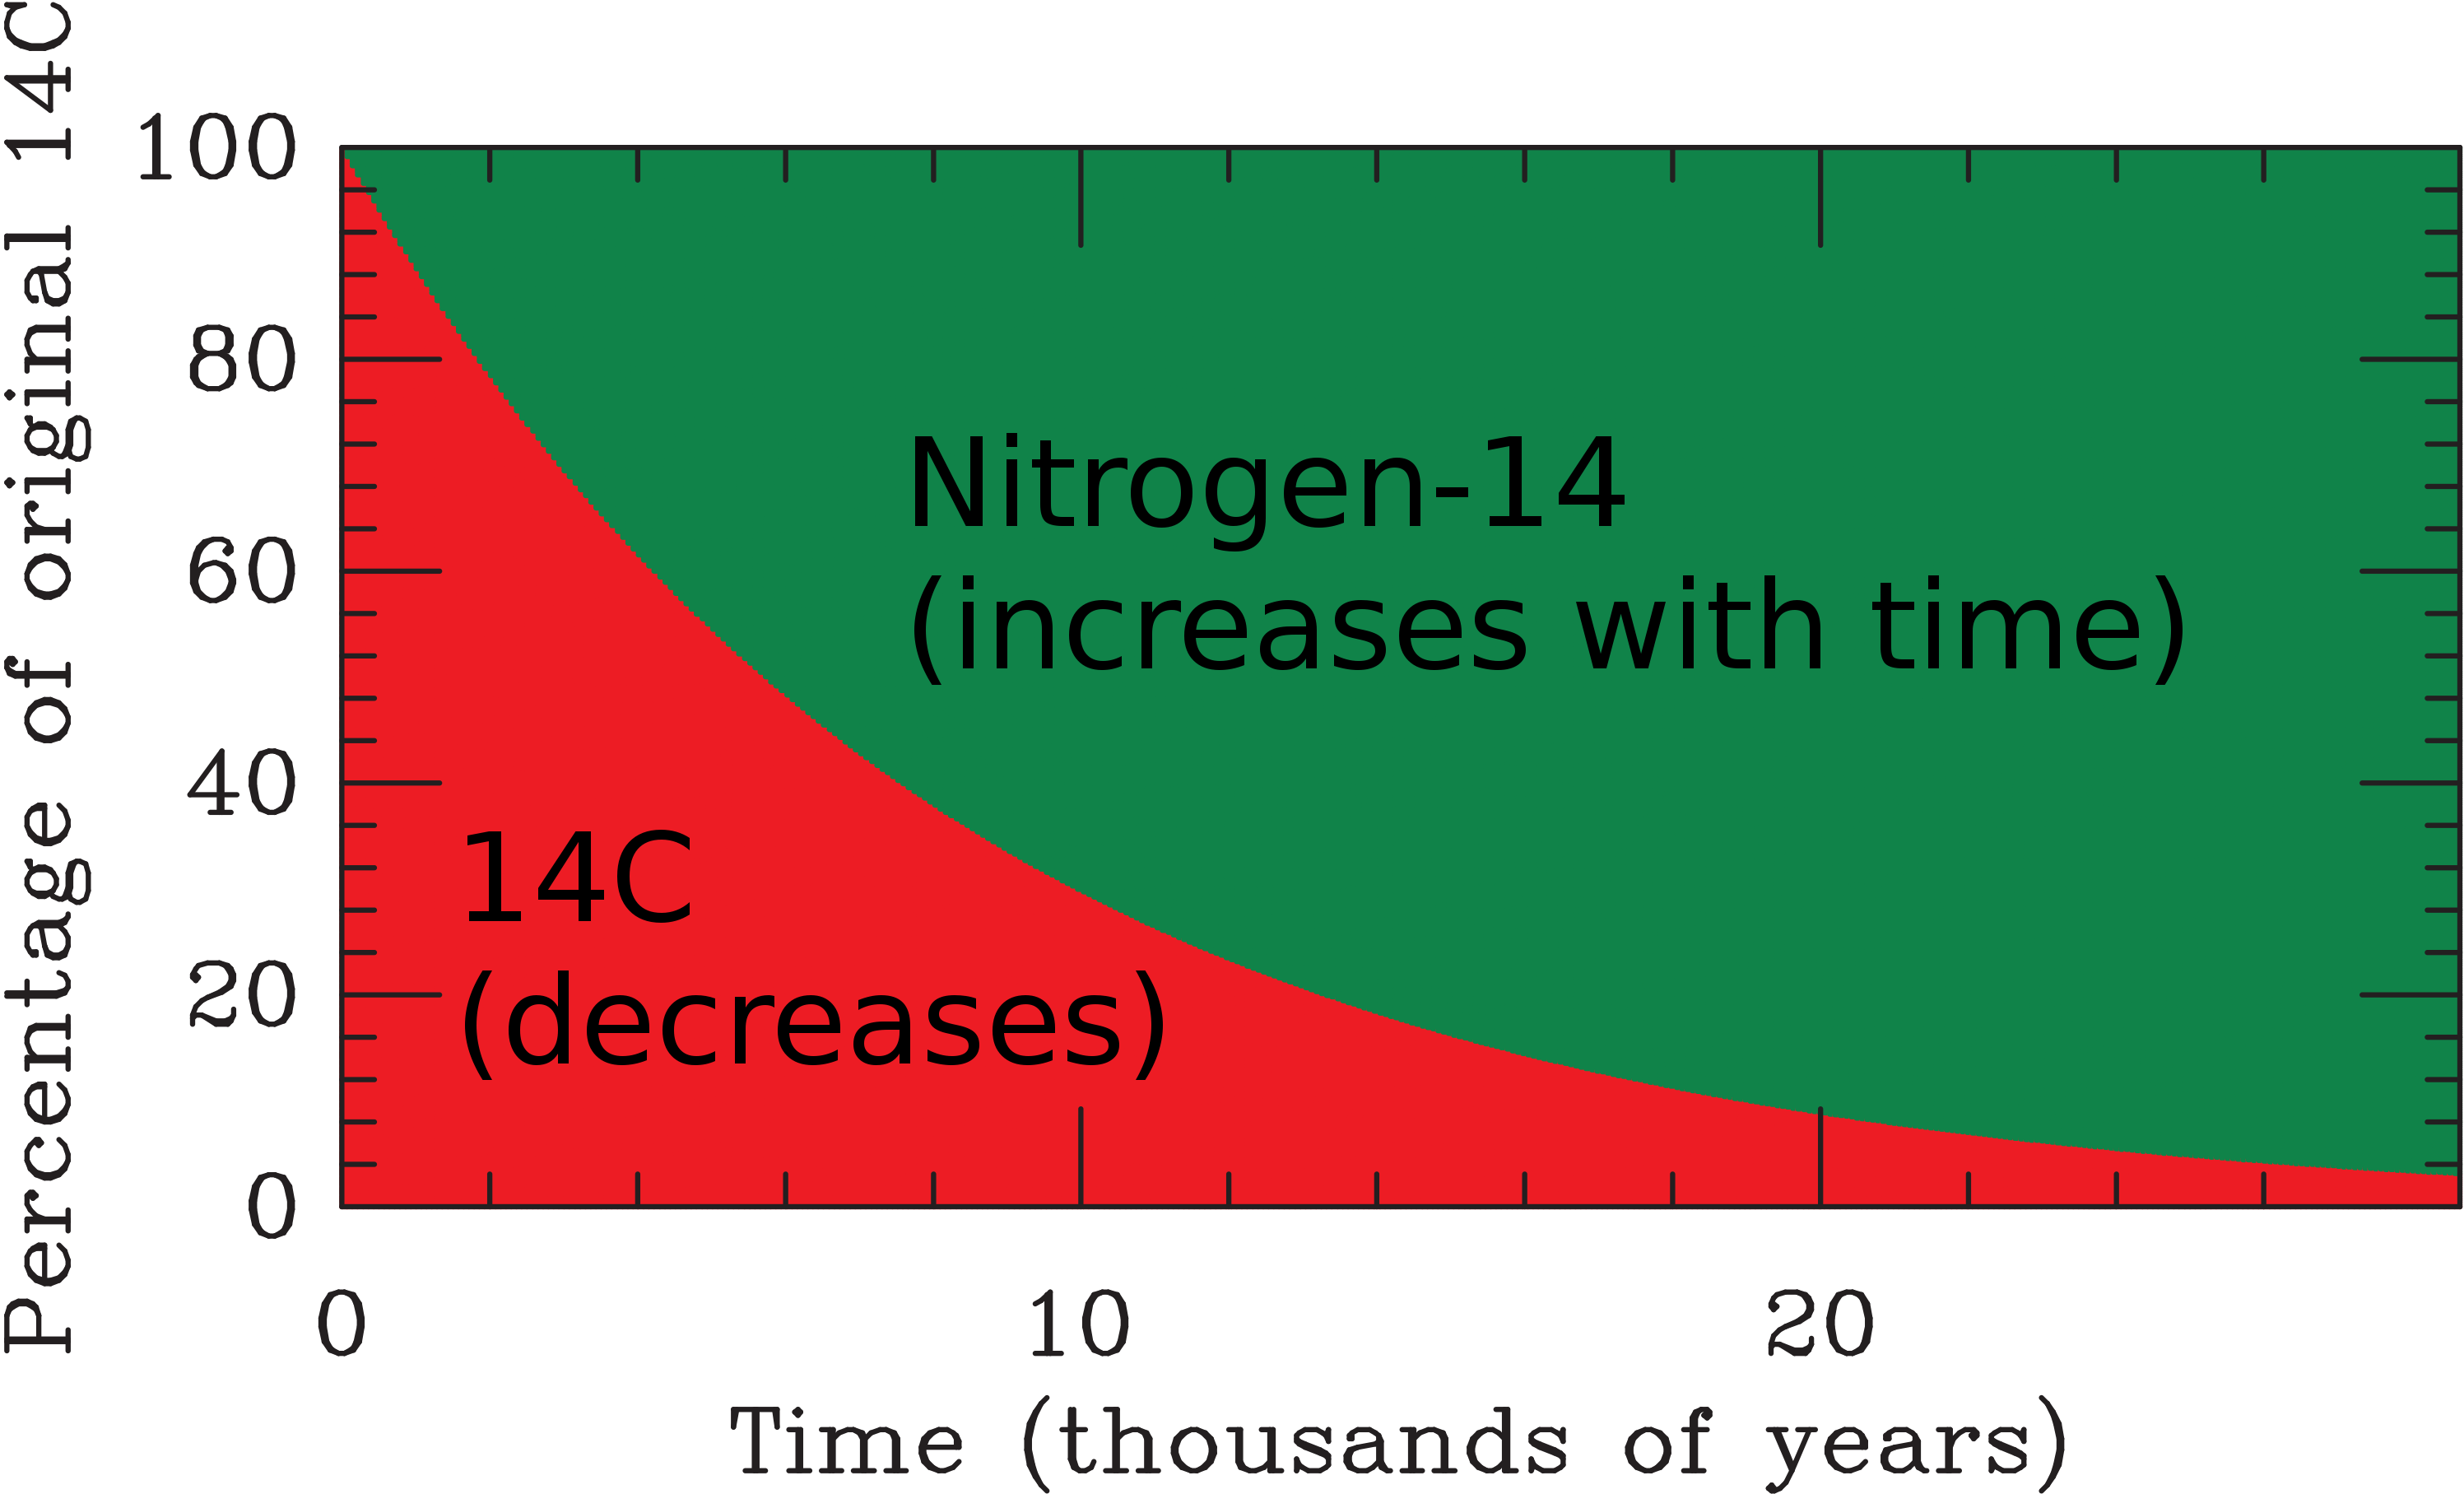
\includegraphics[width=4in]{carbon-fraction-crop.png}
\end{center}

{\bf Question 1:} From the graph, how long did it take for half of the carbon-14 to turn into nitrogen-14? This is the half-life.

\vspace{1in}

{\bf Question 2:} How long will it be until only 1/4 of the original sample is made of carbon-14? How many ``half-lives'' is this?

\vspace{1in}

{\bf Question 3:} How long will it be until only 1/8 of the original sample is made of carbon-14? How many ``half-lives'' is this?

\vspace{1in}

{\bf Question 4:} Suppose you have a sample that is almost completely gone. You measure it and see that only 1/32 of the original
${}^{14}\rm C$ atoms are left. How old is it? This is the principle behind carbon dating: by determining the fraction of the original ${}^{14}\rm C$ that is left, we can estimate how old something is.

\vspace{1in}

\section{Simulating radioactive decay}

One of the more counterintuitive ideas here is that the decay of individual atoms is random, but the rate of decay of large collections
of atoms can be very predictable. To simulate this, we have lots of dice. Count all of your dice, and then repeat the following:

\begin{itemize}
\item Roll all your dice.
\item Remove all the dice that come up 1.
\item Add a point to the graph paper and data table (included later) 
\item As you do so, go to the Lab 10 Data Google Form (linked from the course website, or at \url{https://bit.ly/2DeviP1}) and enter your data there as well.
\end{itemize}

It is okay if you maintain only one data table and one graph for your group, but it is everyone's responsibility to make sure that they are accurate and to help take data!

Once you're finished (all the dice are gone), connect the dots on your graph with a straightedge. This will let you determine the half-life of your dice with more precision. For instance, if you started with 120 dice, and there were 65 left after 3 rolls and 55 after 4 rolls,
the line between these two points would cross the ``60'' line between 3 and 4. Thus you might conclude that half of the dice ``decayed'' after 3.5 rolls. This procedure of connecting the dots to get more precise estimates is called 
``interpolation'' in mathematics. Once you have your graph, show it to your TA.

{\bf TA should sign below if everyone in this group was involved in taking data:}



\newpage
{\bf Question 5:} How many rolls did it take for your dice to decay from 120 to 60? This will give you an estimate of the half-life of your dice. Remember, based on your interpolation, your answer may be a decimal.

\vspace{1.1in}

{\bf Question 6:} How many rolls did it take for your dice to decay from 60 to 30? This will give you another estimate of the half-life of your dice.


\vspace{1.1in}

{\bf Question 7:} How many rolls did it take for your dice to decay from 30 to 15? This will give you another estimate of the half-life of your dice.


\vspace{1.1in}

{\bf Question 8:} If you were to quote to someone the half-life of your dice in ``rolls'', what would you tell them? How did you determine this based on your answers to the preceding three questions?


\vspace{1.5in}

{\bf Question 9:} Is the decay of your dice smooth and predictable when there are many of them left? What about for the last few? How does this limit the maximum age of objects that can be dated with carbon dating?

\newpage

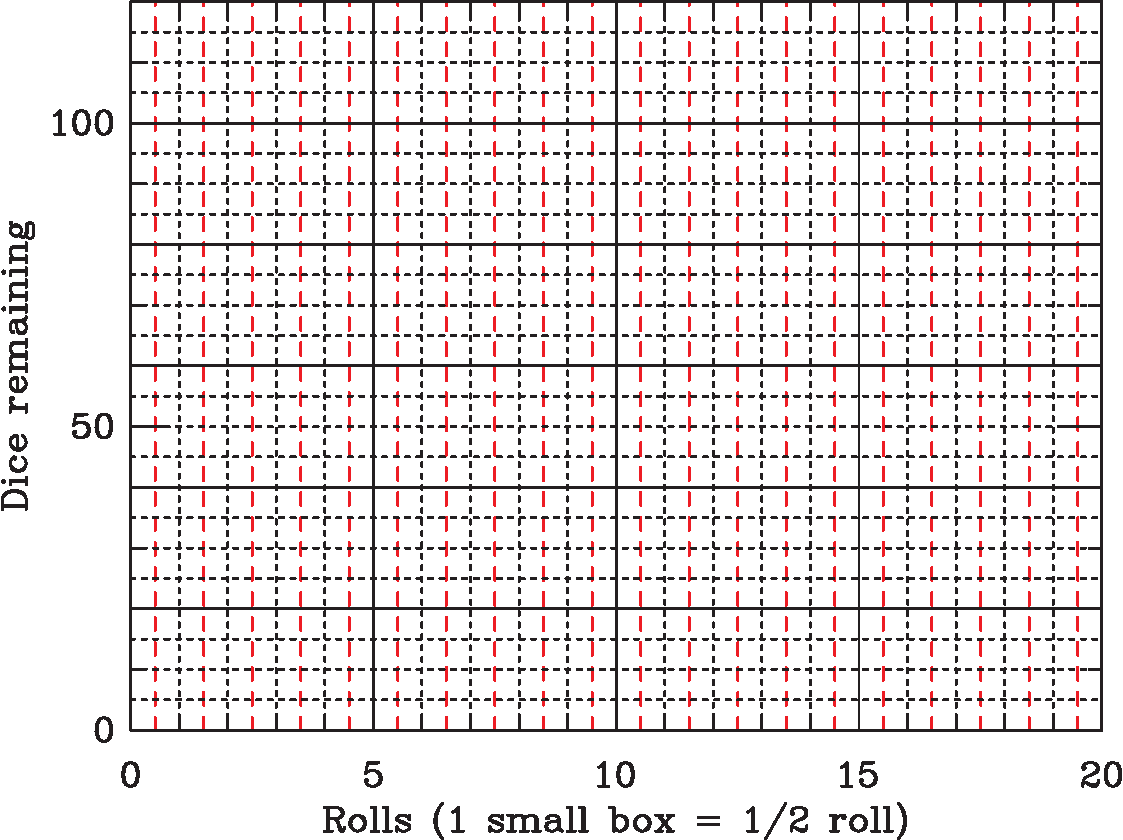
\includegraphics[height=\textwidth,angle=90,origin=c]{graphpaper-crop.pdf}
\newpage
\begin{center}
This page intentionally left blank.
\end{center}
\newpage
\huge
\begin{center}
\begin{tabular}{|c|c|}
\hline
Number of Rolls & Dice Remaining \\ \hline
0               & 120            \\ \hline
1               &                \\ \hline
2               &                \\ \hline
3               &                \\ \hline
4               &                \\ \hline
5               &                \\ \hline
6               &                \\ \hline
7               &                \\ \hline
8               &                \\ \hline
9               &                \\ \hline
10              &                \\ \hline
11              &                \\ \hline
12              &                \\ \hline
13              &                \\ \hline
14              &                \\ \hline
15              &                \\ \hline
16              &                \\ \hline
17              &                \\ \hline
18              &                \\ \hline
19              &                \\ \hline
20              &                \\ \hline
\end{tabular}
\end{center}
\newpage
\begin{center}
\normalsize
This page intentionally left blank.
\end{center}
\newpage
\normalsize
{\bf Question 10:} Suppose someone gives you a bin of dice and asks the following question: {\it ``I started with 200 dice. 
Now I have only 60 of them left. I've forgotten how many times I've rolled them, though, but I did the same thing you did -- I rolled
them and removed all the 1's. All I know is that I started with 200 and I only have 60 left now. Can you help me figure out about how many times I've rolled them all?''} 
What would you tell them?


\vspace{2in}

\section{The age of the Earth}

In order to date the Earth, we need isotopes with much longer half-lives. Two of these are uranium-235 (which decays into lead-207) and potassium-40 (which decays into argon-40). The age of the Earth has been measured with these radioactive decays,
as well as others. For this lab, let's think about the decay of uranium-235 into lead-207 with a half-life of 710 million years.

A type of rock called {\it zircon} sometimes forms with uranium atoms included in it, but does not include lead. 

{\bf Question 11:} Suppose that you find a zircon crystal that includes lead atoms inside it. You know that they could not have formed inside the zircon, because of its chemistry. 
How did they get there, and what can you conclude about the time that this zircon crystal formed?

\vspace{2in}

\newpage
{\bf Question 12:}
Geologists have found zircon crystals all around the world like this. Suppose that you find such a crystal, and there are fifteen lead-207 atoms for every uranium-235 atom inside the zircon. How long ago
did this rock form? 

If you are stuck on this problem, retrace the history of the uranium-235 and lead-207 in this crystal in the following table. I've filled out the first two rows for you:

\Large
\begin{tabular}{|l|l|l|l|l|}
\hline
Half-lives & Years elapsed & ${}^{238}\rm U$ fraction & ${}^{207}\rm Pb$ fraction & Schematic of atoms                          \\ \hline
0                                   & 0                              & 16/16                                            & 0/16                                          & {\tt UUUUUUUUUUUUUUUU} \\\hline
1                                   & 710 million                    & 8/16                                             & 8/16                                          & {\tt LLLLLLLLUUUUUUUU} \\\hline
2                                   &                                &                                                  &                                               &                                             \\\hline
3                                   &                                &                                                  &                                               &                                             \\\hline
4                                   &                                &                                                  &                                               &                                             \\\hline
\end{tabular}

\normalsize\vspace{1.5in}

{\bf Question 13:} The oldest zircon crystals that we find have around sixty-three lead-207 atoms for every uranium-235 atom; in other words, the
compostion of these two atoms, taken together, is 63/64 lead-207 and 1/64 uranium-235.
 About how old are they? This gives us an estimate of the age when the Earth's surface cooled enough to form rocks like 
zircon. (It is actually a few hundred million years older than this; I rounded off to a 63:1 ratio to make it easier to do the math.)

\vspace{1.2in}

{\bf Question 14:} When we apply radioactive dating to asteroids that fall to Earth, rocks from the Moon, and the surface of Mars (using robots), we get the same value: around 4.5 billion years old. Is this consistent with a model of solar system formation where the Sun and all the planets formed from the same cloud of gas and dust? Explain.

\vspace{1.5in}
\newpage

{\bf Question 15:} There are actually {\it two} naturally-occurring isotopes of uranium: uranium-235, with a half-life of 710 million years, and uranium-238, with a half-life of 4.5 billion years. These are found mixed together in nature, since they have the same chemical properties.

Currently, natural uranium is almost entirely $\null^{238}$U. Only 0.7\% of natural uranium is $\null^{235}$U. Billions of years ago, much earlier in Earth's history, would the fraction of $\null^{235}$U be higher or lower than 0.7\%? How do you know?

\vspace{2in}

{\bf Question 16:} Only $\null^{235}$U can participate in nuclear fission chain reactions like those used in nuclear power plants; $\null^{238}$U is not fissile.

A mixture of uranium and water can sustain a nuclear chain reaction if the fraction of $\null^{235}$U is above 2.5\%. Geologists have discovered that this happened naturally a long time ago: a deposit of uranium mixed with water ``went critical'' in the same way that power plants do near Oklo, Gabon.

Estimate how long in the past this must have happened. (Hint: The current fraction of $\null^{235}$U is 0.7\%. Given the half-life of around 700 million years for $\null^{235}$U, when would the fraction have been over 2.5\%?)

\vspace{3in}

\large

{\bf Before you leave, gather your dice back up and arrange them into a 12x10 block on your table. If there aren't 120 of them, let your TA know; we have a few spares.}

\end{document}
